\documentclass[crop,border=7pt]{standalone}
\usepackage{tikz}
\usepackage{ifthen}
\usetikzlibrary{shapes.geometric}
\begin{document}

 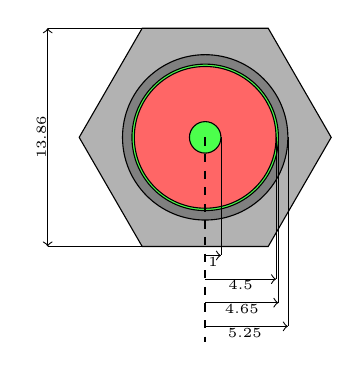
\begin{tikzpicture}[scale=0.2]
  
%%%hexagon 1
\newdimen\R
\R=8.002cm
  \coordinate (center) at (0,0);
 \filldraw[gray!60, draw=black,thin] (0:\R)
     \foreach \x in {60,120,...,360} {  -- (\x:\R) }
              -- cycle (300:\R)
              -- cycle (240:\R) 
              -- cycle (180:\R) 
              -- cycle (120:\R) 
              -- cycle (60:\R) 
              -- cycle (0:\R) ;
              
              
              %%%%pins
			\filldraw[gray, draw=black] (0,0) circle (5.25cm);
			\filldraw[green!70, draw=black]  (0,0) circle (4.65cm);
			\filldraw[red!60, draw=black]  (0,0) circle (4.5cm);
			\filldraw[green!70, draw=black]  (0,0) circle (1.0cm);
%               
%%%%%%%%%
 %%%%%%asse
\draw[black, thick, dashed] (0,0) -- (0,-13);
%%%%%quote totale
\draw[black, very thin] (5.25, 0) -- (5.25,-12);
\draw[black, thin, ->] (0,-12) -- (5.25,-12);
\draw[black] (2.5125,-11.5) node[anchor=north] {\tiny 5.25};
%%%%%%%
\draw[black, very thin] (4.65, 0) -- (4.65,-10.5);
\draw[black, thin, ->] (0,-10.5) -- (4.65,-10.5);
\draw[black] (2.325,-10) node[anchor=north] {\tiny 4.65};
%%%%%%%
\draw[black, very thin] (4.5, 0) -- (4.5,-9);
\draw[black, thin, ->] (0,-9) -- (4.5,-9);
\draw[black] (2.25,-8.5) node[anchor=north] {\tiny 4.5};
  %%%%%%%
\draw[black, very thin] (1,0) -- (1,-7.5);
\draw[black, thin, ->] (0,-7.5) -- (1,-7.5);
\draw[black] (0.5,-7) node[anchor=north] {\tiny 1};

%%%%%%%%%%%%%%%%%%%%%%%%%%%%%%%%55  
\draw[black, very thin] (-3, 6.92994) -- (-10,6.92994);
\draw[black, very thin] (-3, -6.92994) -- (-10,-6.92994);
\draw[black, thin, <->] (-10,6.92994) -- (-10,-6.92994);
\draw[black] (-9.5,0) node[anchor=south, rotate=90] {\tiny 13.86};
% \draw[black] (2.5125,-11.5) node[anchor=north] {\tiny 5.25};

  \end{tikzpicture}
\end{document}